\documentclass[a4paper,12pt]{article}
\usepackage[latin1,utf8]{inputenc}
\usepackage[portuguese]{babel}
\usepackage{color}
\usepackage{graphicx}
\usepackage{ulem}
\title{A vida do Suricata}
\author{João António-dos-Santos}
\date{\today}
\begin{document}
\maketitle
\section{Sobre o Suricata}
O \textbf{suricata}, também chamado de \textbf{suricato} ou \textbf{suricate} (\textit{Suricata suricatta}) é um pequeno mamífero da família \textit{Herpestidae}, nativo do deserto do Kalahari. Estes animais têm cerca de meio metro de comprimento (incluindo a cauda), em média 730 gramas de peso, e pelagem acastanhada. Têm garras afiadas nas patas, que lhes permitem escavar a superfície do chão e dentes afiados para penetrar nas carapaças quitinosas das suas presas. \textcolor{red}{Outra característica distinta é a sua capacidade de se elevarem nas patas traseiras, utilizando a cauda como terceiro apoio}.
\section{Características gerais}
\subsection{Alimentação}
Alimenta-se principalmente de insetos (cerca de 82\%): larvas de escaravelhos e de borboletas; também ingerem milípedes, aranhas, escorpiões, pequenos vertebrados (répteis, anfíbios e aves), ovos e matéria vegetal. \uline{São relativamente imunes ao veneno} das najas e dos escorpiões, sendo estes, inclusive, um dos alimentos que mais apreciam.
\begin{figure}
\caption{Suricata no Zoo de Lisboa}
\centering
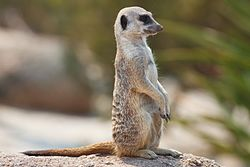
\includegraphics[scale=1.8]{Suricata}
\end{figure}
\end{document}
